%% Estructura principal para un reporte de Trabajos intersemanales CIRCAE %%
\documentclass[a4paper]{IEEEtran} %tamaño del papel y el tipo de transcripción que será IEEE
\usepackage[utf8]{inputenc} %el tipo de codificación que incluye símbolos como la tilde
\usepackage[spanish]{babel} % hacemos que nuestro documentación vaya en español
\usepackage{cite} % citas bibliográficas
\usepackage{graphicx} %gráficos, usaremos solo .jpg o .png con estándares que ya veremos
\usepackage{subfigure}
\usepackage{url}
\usepackage{amsmath}
\usepackage{booktabs} 
\providecommand{\keywords}[1]{\textbf{\textit{Términos Clave---}} #1}
\begin{document}
%\tableofcontents%tabla de contenidos
%\listoffigures%lista de figuras
\title{Esquemas de Control Tipo Hiperbólico para Aeropéndulo}
\author{Hanan Ronaldo Quispe Condori, Joel Huamán Zárate, Héctor Lionel García Hurtado, Roly Sandro Gutierrez Benito, María Teresa Vera Percca}
%\markboth{INFORME CIRCAE 2019-08-05-G1-P3-001}{} % Codigo del informe que corresponde a: semestre | mes | dia | numero de grupo con la G antepuesta | numero de proyecto con la P antepuesta | número de informe
\maketitle
\begin{abstract}
    Se propone la aplicación de una familia de esquemas de control tipo hiperbólico de alto desempeño para el problema de control de posición angular del aeropendulo, los metodos de control clasicos resuelven este problema satisfactoriamente en el sistema linealizado mas el enfoque no lineal permite un control preciso sobre toda la dinámica del sistema en mención.
\end{abstract}
\section{Modelamiento Matemático}
\label{sec:modeling}
Se usará el enfoque de dinámica analítica, este enfoque usa las ecuaciones de movimiento de Euler-Lagrange para la obtención del modelo dinámico del sistema, se eligio este metodo debido a que se obtiene una estructura matemática bien definida el cual se integra de manera natural con la teoria de estabilidad de Lyapunov para el análisis de estabilidad para sistemas dinámicos lineales y no lineales sin importar el orden del sistema.[\cite{reyes2019drones}]

Se obtendrá la cinemática directa del sistema en función de la coordenada generalizada $\  theta$.

\begin{equation}
    \begin{bmatrix}  x \\ y \\
    \end{bmatrix}=
    \begin{bmatrix} Lsen(\theta) \\ -L\cos(\theta)  \\
    \end{bmatrix}
    \label{eq:cin_direc}
\end{equation}

Apartir de \ref{eq:cin_direc} se podrá obtener la cinemática diferencial para calcular la rapidez lineal.

\begin{equation}
    \frac{d}{dt}\begin{bmatrix}
        x \\
        y \\
    \end{bmatrix}=
    \begin{bmatrix}
        \dot{\theta}L\cos(\theta)  \\
        \dot{\theta}L\sen(\theta)  \\
    \end{bmatrix}
    \label{eq:speed}
\end{equation}

La rapidez lineal esta dada por

\begin{equation}
    \begin{split}
        \|v\|^2&=v.v^T=\sqrt{\dot{\theta}^2L^2sen^2{\theta}+\dot{\theta}^2L^2cos^2{\theta}}^2\\
        \|v\|^2&=L^2\dot{\theta}^2
    \end{split}
    \label{eq:speed_mod}
\end{equation}

Usando la expresión de la rapidez lineal del sistema se procedera a calcular el modelo de energía del sistema.

\begin{equation}
    \begin{split}
        \mathcal{K}(\theta,\dot{\theta}) &= \frac{1}{2}mL^2\dot\theta^2\\
        \mathcal{K}(\theta,\dot{\theta}) &= \frac{1}{2}J\dot\theta^2\\
        \mathcal{U}(\theta) &=  -m_1g\frac{L}{2}\cos{\theta} -m_2gL\cos{\theta} \\
        \mathcal{U}(\theta) &= -gL\cos{\theta(\frac{m_1}{2}+m_2)}
    \end{split}
    \label{eq:energy}
\end{equation}

El lagrangiano del sistema esta dado por
\begin{equation}
    \begin{split}
        \mathcal{L}(\theta,\dot{\theta})=\mathcal{K}(\theta,\dot{\theta})-\mathcal{U}(\theta)=\frac{1}{2}J\dot{\theta}^2+gL\cos{\theta}(\frac{m_1}{2}+m_2)
    \end{split}
    \label{eq:lagrange}
\end{equation}

Las ecuaciones de Euler lagrange para el sistema tienen la siguiente forma

\begin{equation}
    \frac{d}{dt}\begin{bmatrix}
        \frac{\partial \mathcal{L}(\theta,\dot{\theta})}{\partial\dot{\theta}}
    \end{bmatrix}-\begin{bmatrix}
        \frac{\partial \mathcal{L}(\theta,\dot{\theta})}{\partial \theta}
    \end{bmatrix}+f_f(f_e,\dot{\theta})=\tau
    \label{eq:eu_lagran}
\end{equation}

Usando el lagrangiano se tienen las siguientes expresiones

\begin{equation}
    \begin{split}
        \begin{bmatrix}
            \frac{\partial \mathcal{L}(\theta,\dot{\theta})}{\partial\dot{\theta}}
        \end{bmatrix}&=J\dot{\theta}\\
        \frac{d}{dt}\begin{bmatrix}
            \frac{\partial\mathcal{L}(\theta,\dot{\theta})}{\partial\dot{\theta}}
        \end{bmatrix}&=J\ddot{\theta}\\
        \begin{bmatrix}
            \frac{\partial \mathcal{L}(\theta,\dot{\theta})}{\partial \theta}
        \end{bmatrix}&=-Lg\sen(\theta)(m_2 + \frac{m_1}{2})\\
    \end{split}
    \label{eq:dq}
\end{equation}

El modelo dinámico del sistema considerando el fenomeno de fricción esta dado por:

\begin{equation}
    J\ddot{\theta}+Lg\sen(\theta)(m_2+\frac{m_1}{2})+c\dot{\theta}=\tau
    \label{eq:din_model}
\end{equation}

Además del modelo dinámico del pendulo tambien se tendrá que obtener un modelo dinámico del rotor, esto para obtener un modelo que describa en su totalidad el comportamiento físico del sistema.



\section{Fundamento Teórico}
\label{sec:fundamento}
Los divisores de potencia son caracterizados por matrices de dispersión que nos diran cual sera el comportamiento de dicho divisor, esta matriz es cuadrada cuyo orden dependerá del numero de puertos utilizados en nuestro caso sera de orden 3, ademas de ello si se analizan sus propiedades podremos saber si esta pertenece a un acoplador, divisivor de potencia y las carateristicas de los puertos de estas\cite{pozar2012microwave}. El divisor de potencia de Wilkinson es un dispositivo en el que todos los puertos estan emparejados, aunque sea un dispositivo de N puertos, normalmente lo encontramos como un divisor de 2 vias(3 puertos),no tiene perdidas cuando se excita el puerto de entrada y los puertos de salida se mantienen aislados.
\vspace{5mm}
\begin{equation}
[S]=
\begin{pmatrix}
S_{11}&S_{12}&S_{13}\\
S_{21}&S_{22}&S_{23}\\
S_{31}&S_{32}&S_{33}\\
\end{pmatrix}
\label{eq:scattering}
\end{equation}
Scattering matrix \ref{eq:scattering}.
\vspace{5mm}

Para analizar totalmente esta estructura realizaremos un análisis de modo par-impar, para dicho análisis partiremos el divisor de potencia como se muestra en la figura \ref{fig:Analisis}.
\vspace{50mm}
\begin{figure}[h]
    \centering
        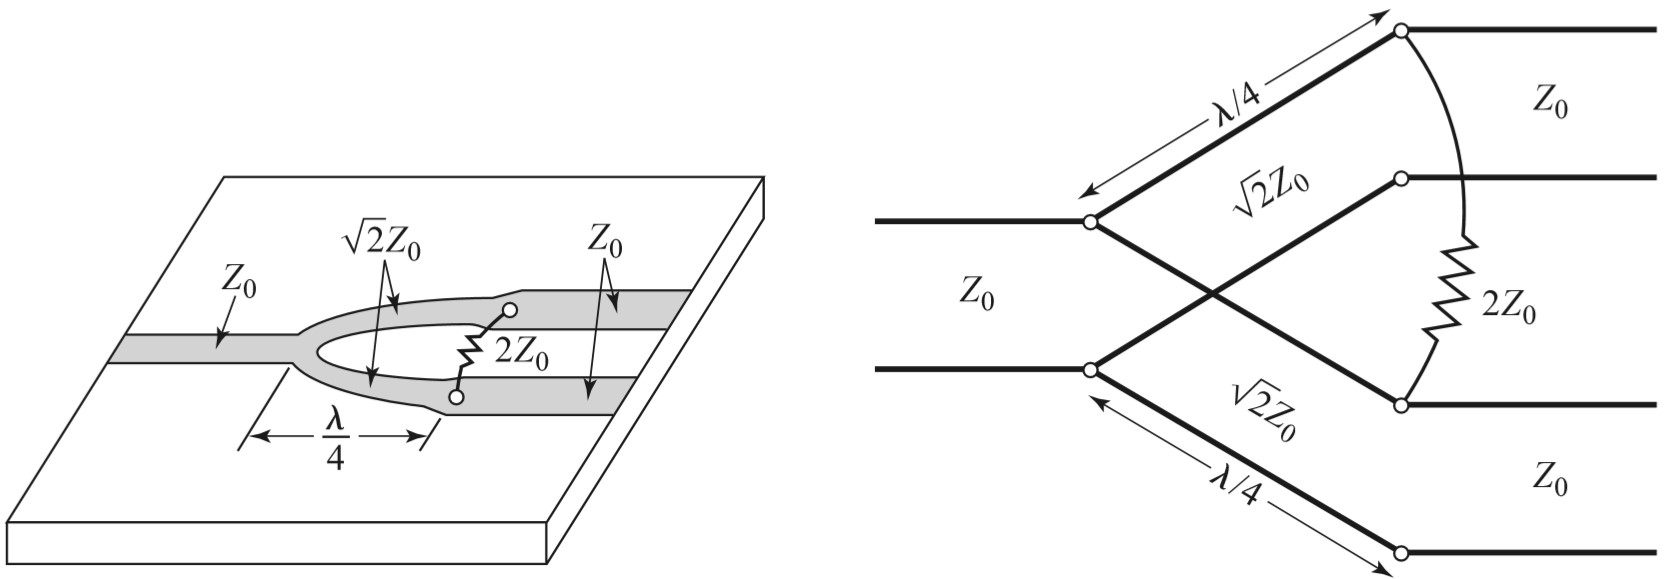
\includegraphics[width=8cm]{imagenes/img17}
        \caption{Division del divisor de potencia de Wilkinson}
        \label{fig:Analisis}
\end{figure}
\begin{figure}[h]
    \centering
    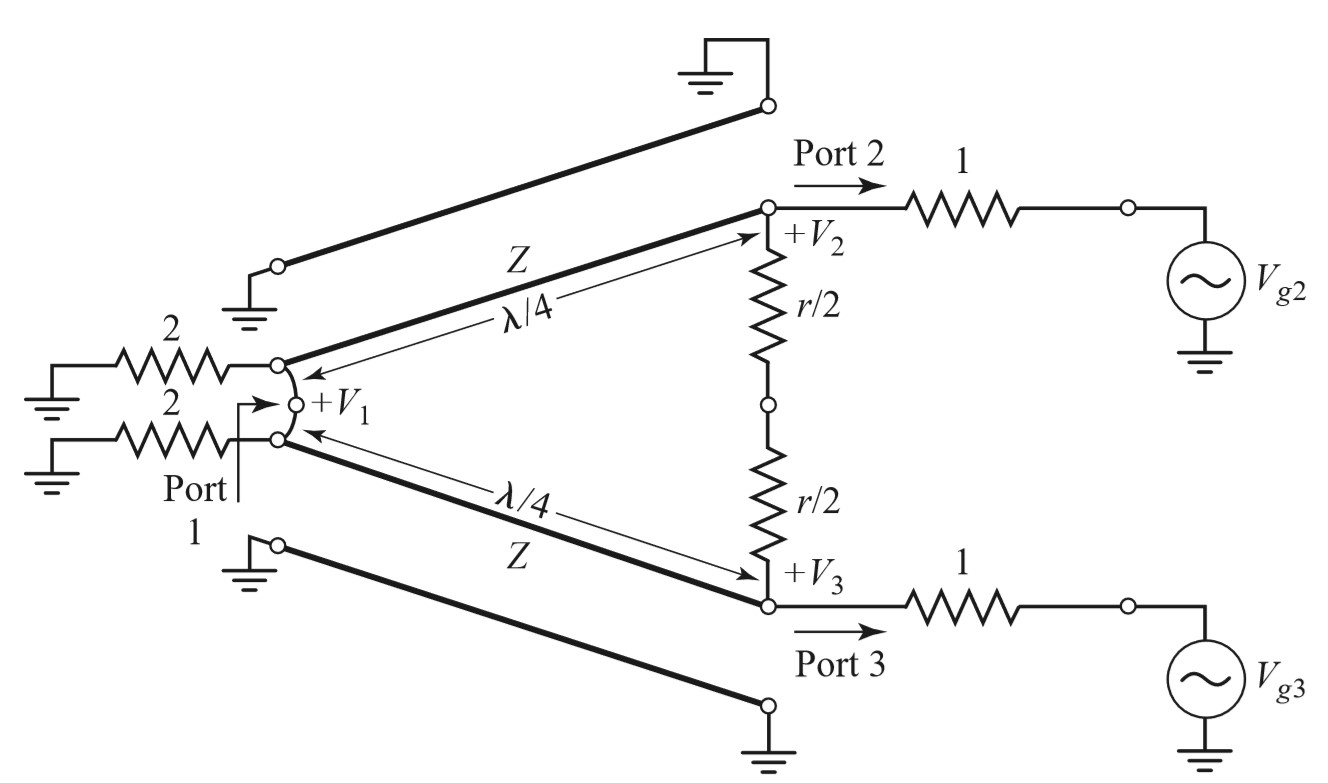
\includegraphics[width=8cm]{imagenes/img3}
    \caption{Diagrama Esquematico del divisor de potencia de Wilkinson.}
    \label{fig:diagrama}
\end{figure}
\begin{figure}[h]    
    \centering
        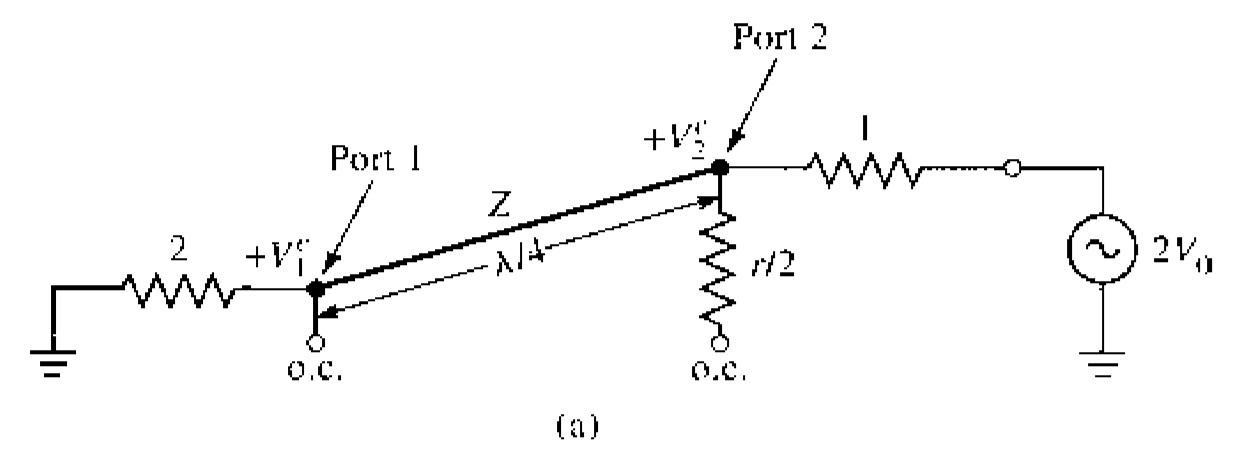
\includegraphics[width=8cm]{imagenes/img4}
        \caption{Analisis Par-Impar.}
        \label{fig:analisis-par-impar}
\end{figure}
Posteriormente como resultado de este análisis tendremos los siguientes parametros de dispersión. 
\begin{equation}
\begin{split}
    S_{11}&=0 \\
    S_{22}&=S_{33}=0 \\
    S_{12}&=S_{21}=-\frac{j}{\sqrt{2}}\\
    S_{13}&=S_{31}=-\frac{j}{\sqrt{2}}\\
    S_{23}&=S_{32}=0
\end{split}
    \label{eq:parametros}
\end{equation}
La matriz de dispersión del modelo que se simulará es la siguiente
\begin{equation}
    \begin{pmatrix}
    0&-\frac{j}{\sqrt{2}}&-\frac{j}{\sqrt{2}}\\
    -\frac{j}{\sqrt{2}}&0&0\\
    -\frac{j}{\sqrt{2}}&0&0\\
    \end{pmatrix}
    \label{eq:matrix_numbers}
\end{equation}
\section{El modelo}
Se utilizará CST Studio Suite para el modelamiento de este divisor, los parametros a utilizar en la simulación estan dados en el cuadro \ref{tab:parametros_simulacion} \cite{cstpage}.
\begin{table}[h]
    \caption{Tabla de Parametros}
\begin{tabular}{@{}lll@{}}
\toprule
Parametro & Valor    & Descripción \\ \midrule
h         & 1.2 mm   & Grosor del Substrato \\
eps\_r    & 4.3      & Permitividad del Substrato \\
t         & 0.035 mm & Espesor de metalización \\ 
W50       & 2.35 mm  & 50 Ohms (Z0) Anchura de linea \\
W70       & 1.23 mm  & 70.71 Omhs (Z0$\sqrt{2}$) \\
l70       & 42.54 mm & Longitud de Lambda / 4 del ancho de línea Z0$\sqrt{2}$\\ \bottomrule
\end{tabular}
\label{tab:parametros_simulacion}
\end{table}

Procederemos a abrir CST Studio Suite, usaremos la plantilla de Planar Coupler and Divider, en modo time domain solver y configuraremos los monitores de campo eléctrico, magnético y flujo de potencia, que usaremos para visualizar los resultados de la simulación.
Seguidamente ingresaremos los parametros de la tabla \ref{tab:parametros_simulacion} como se muestra en la figura.

\begin{figure}[h]    
    \centering
        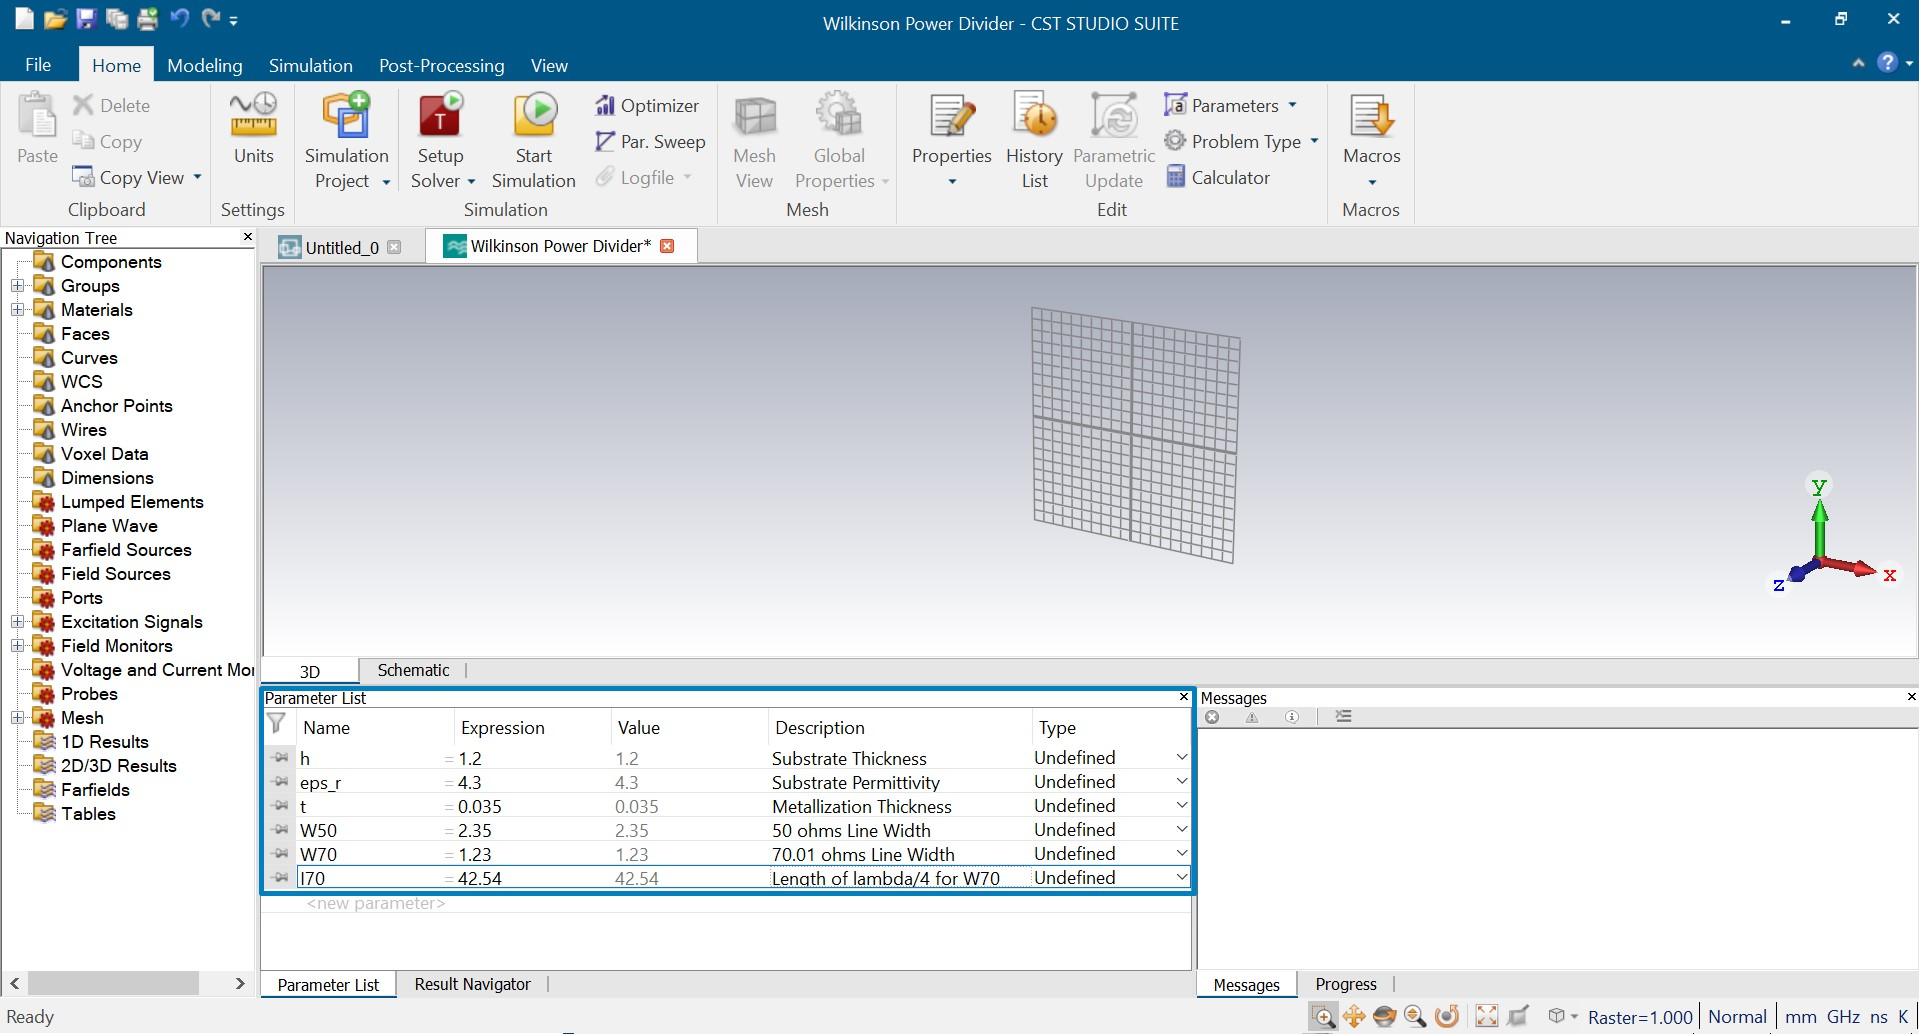
\includegraphics[width=9cm]{imagenes/img5}
        \caption{Ingreso de Parametros de Simulación.}
        \label{fig:ingreso_de_parametros}
\end{figure} 
Una vez los parametros esten ingresados podremos usar sus valores usando sus nombres en cualquier momento de la simulación.

Usaremos los parametros para empezar a construir el divisor de potencia, utilizaremos las herramientas para modelado 3D y las transformaciones disponibles para lograr la geeometria deseada, se muestran imagenes de este proceso.

\begin{figure}[h]    
    \centering
        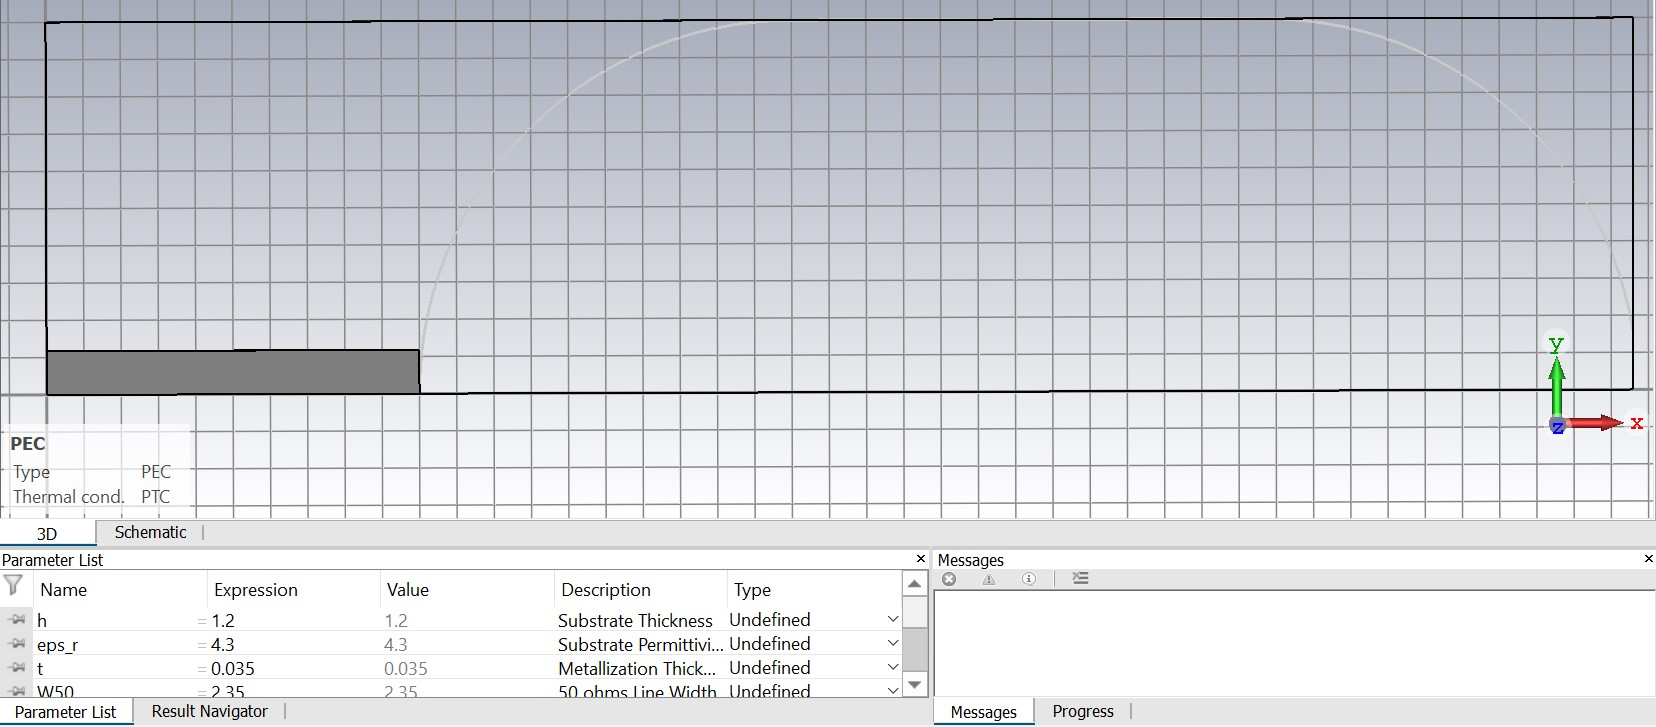
\includegraphics[width=9cm]{imagenes/img6}
        \caption{Construcción del conductor de cobre.}
        \label{fig:modelamiento1}
\end{figure} 
\vspace{50mm}
\begin{figure}[h]    
    \centering
        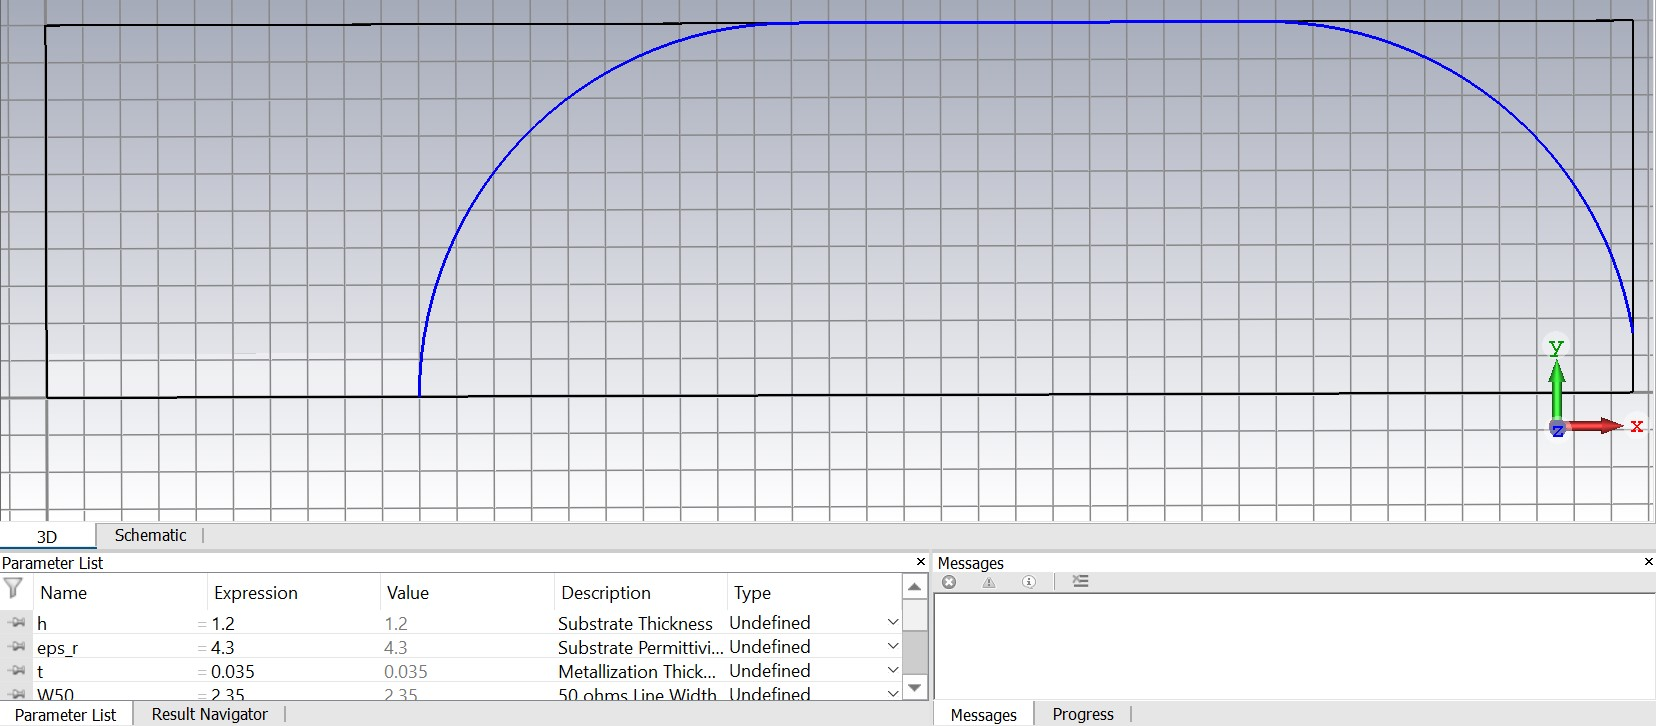
\includegraphics[width=9cm]{imagenes/img7}
        \caption{Construcción del conductor de cobre.}
        \label{fig:modelamiento2}
\end{figure} 
\begin{figure}[h]    
    \centering
        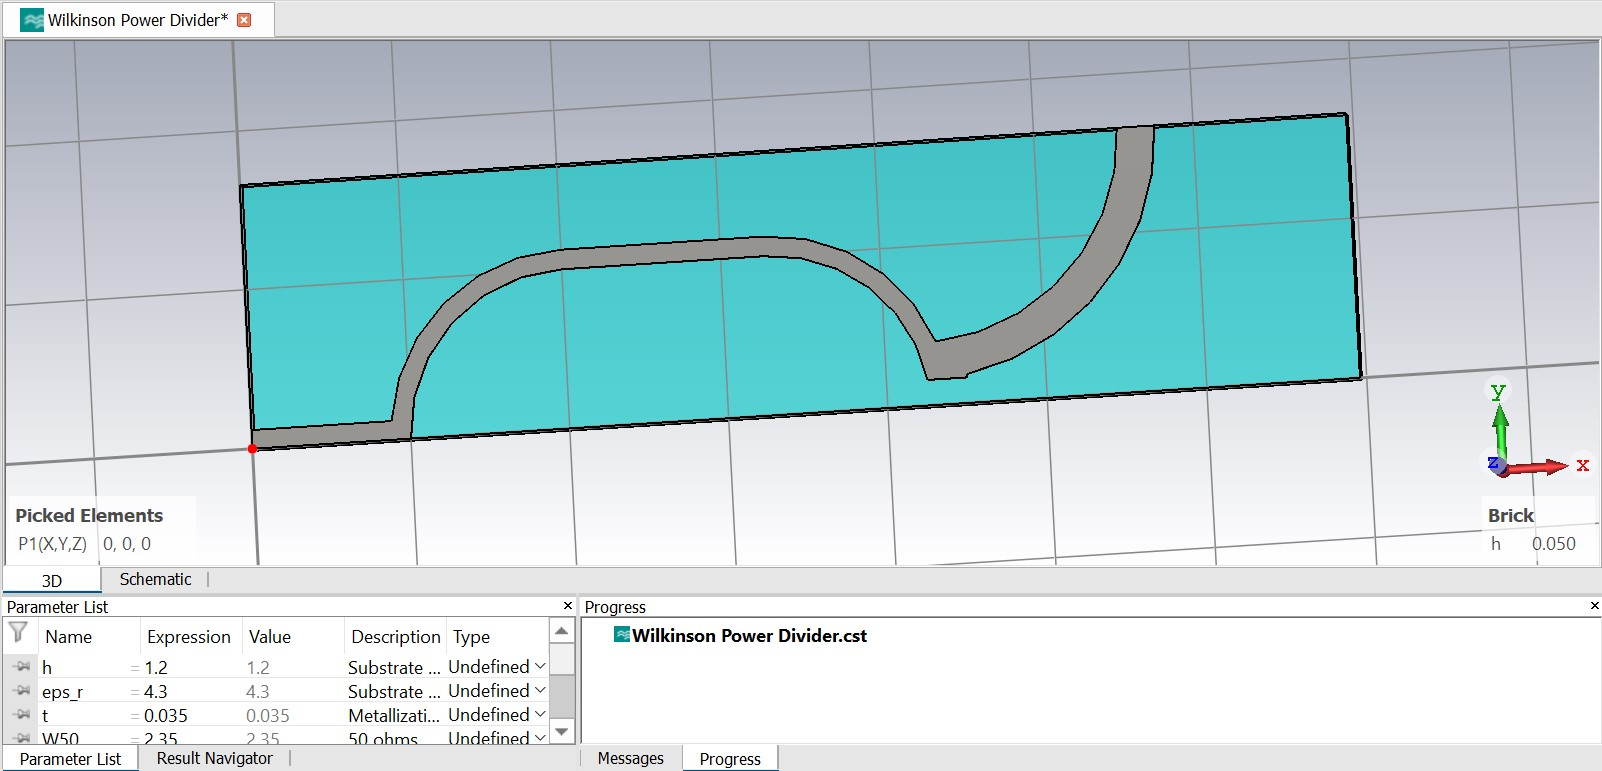
\includegraphics[width=9cm]{imagenes/img8}
        \caption{Construcción de primera mitad con el substrato incluido.}
        \label{fig:modelamiento3}
\end{figure} 

Se aprovechará la simetria del modelo para su construcción, gracias a esto, solo será necesario construir una mitad del divisor y aplicar la transformación del espejo para construir la otra mitad. La línea de entrada es de 50 Omhs. 
\begin{figure}[h]    
    \centering
    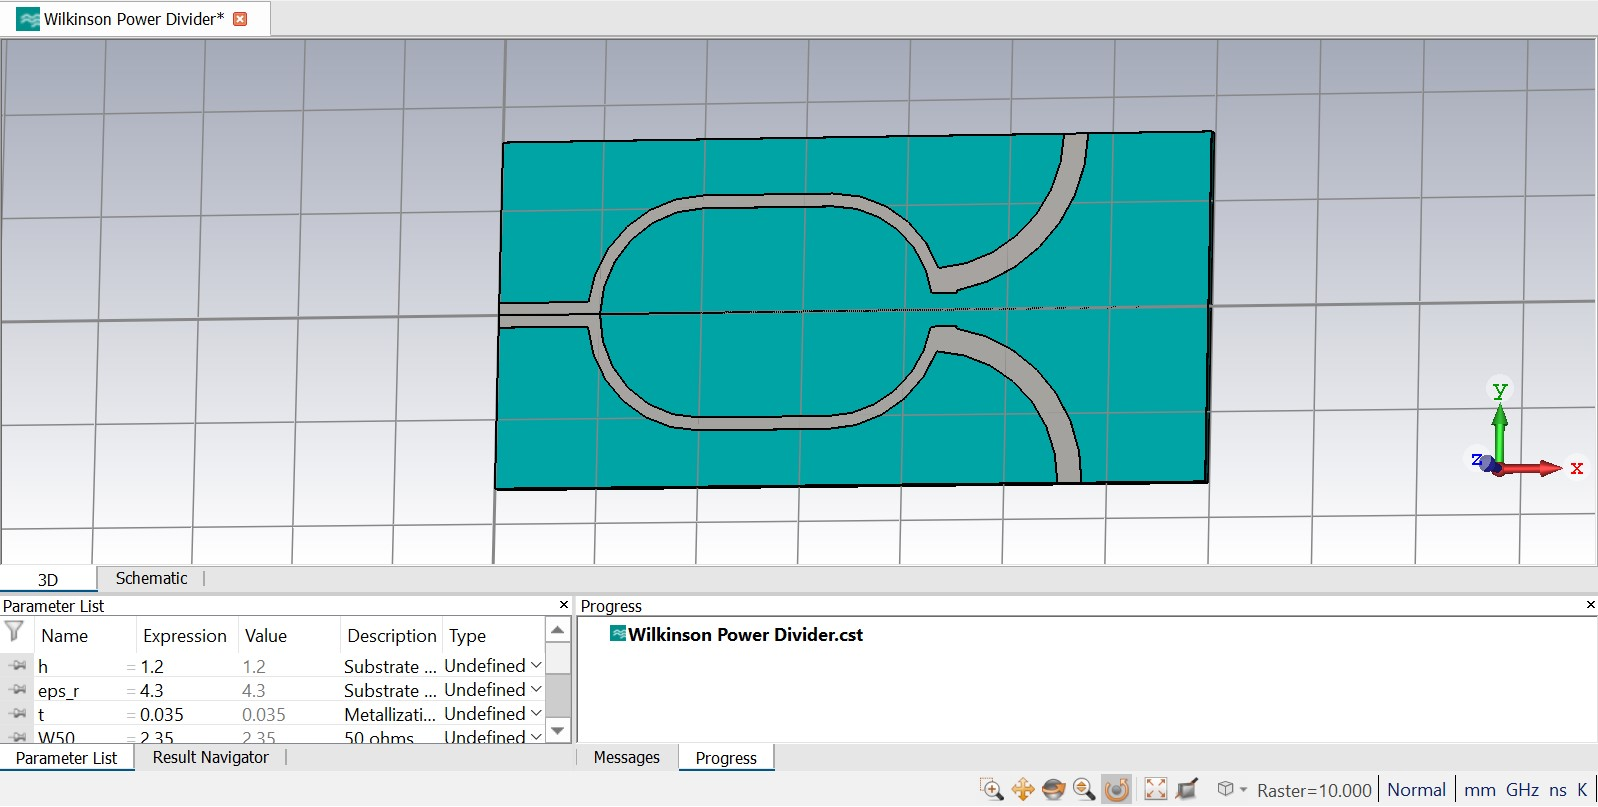
\includegraphics[width=9cm]{imagenes/img9}
    \caption{Uso de la Transformación espejo.}
    \label{fig:modelamiento4}
\end{figure} 
%\vspace{15mm}

Se incluirá una resistencia SMD de 100 Ohms entre las ramas del divisor, esto se muestra en la figura \ref{fig:modelamiento5}.
\begin{figure}[h]    
    \centering
    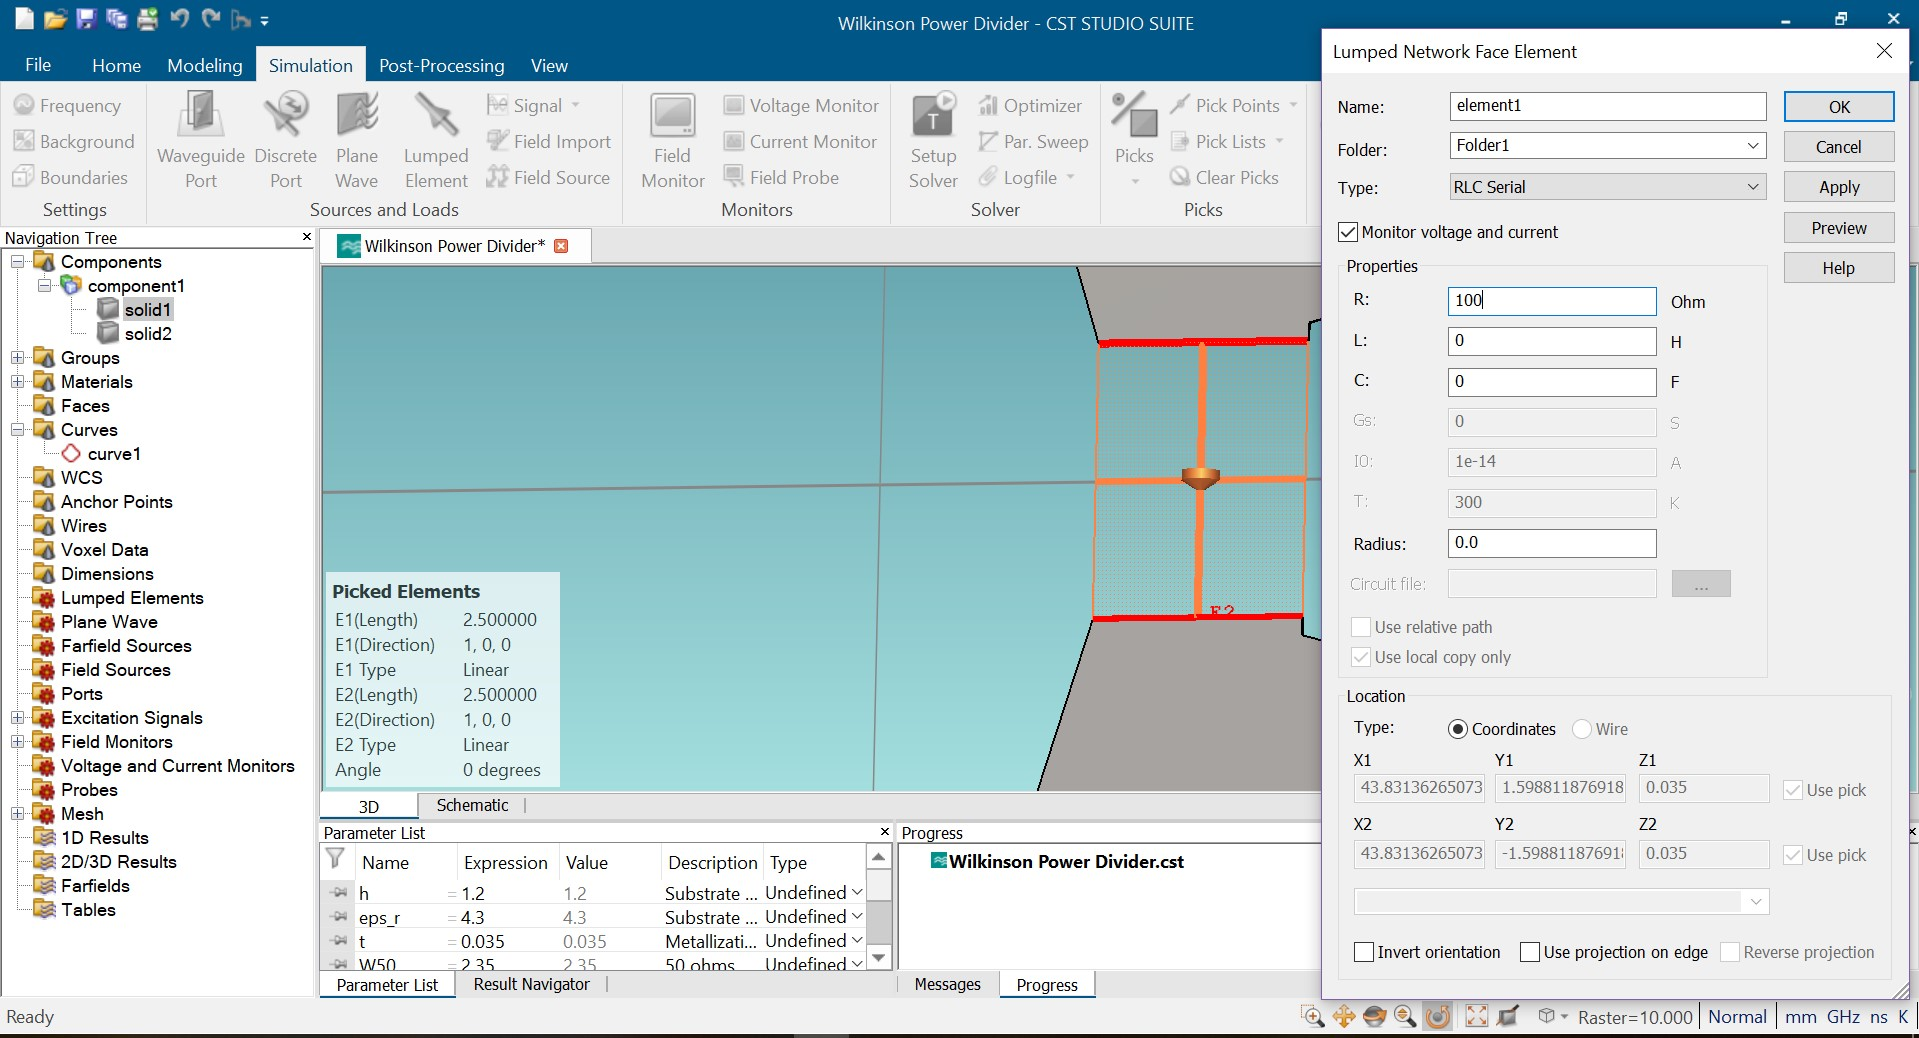
\includegraphics[width=9cm,height=3.403cm]{imagenes/img10}
    \caption{Inclusion del componente SMD.}
    \label{fig:modelamiento5}
\end{figure} 
%\vspace{25mm}

Se configurarán los puertos del divisor, esto se muestra en la figura \ref{fig:modelamiento6}.
\begin{figure}[h]    
    \centering
    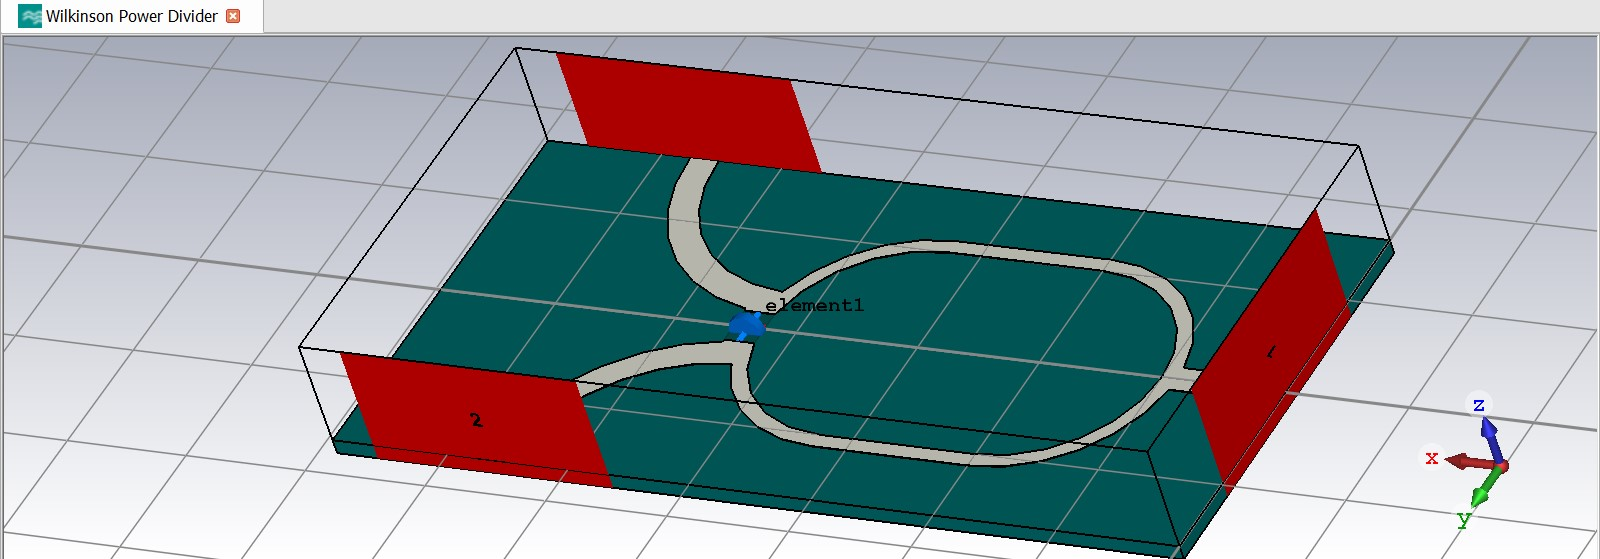
\includegraphics[width=9cm]{imagenes/img11}
    \caption{Modelo terminado.}
    \label{fig:modelamiento6}
\end{figure}
%\vspace{25mm}

Finalmente configuraremos los parametros del solver en el dominio del tiempo para ejecutar la simulación.
\begin{figure}[h]    
    \centering
    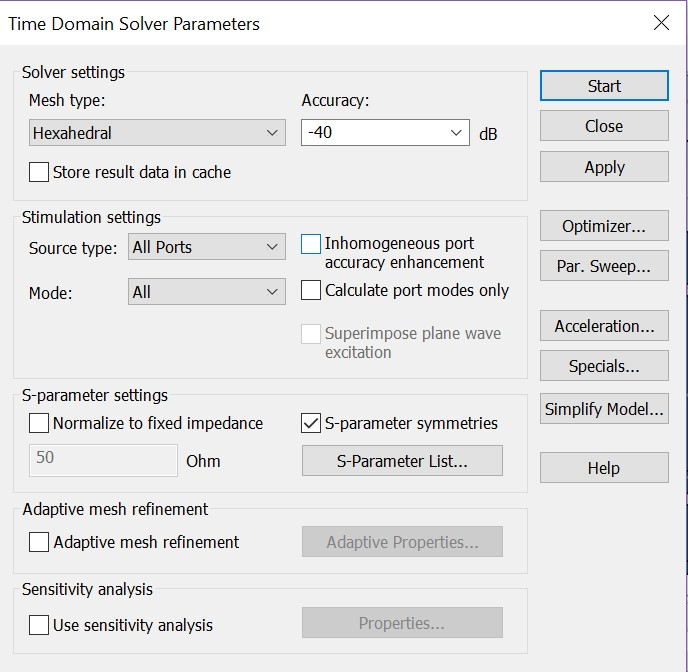
\includegraphics[width=9cm]{imagenes/img12}
    \caption{Parametros de Simulación.}
    \label{fig:modelamiento7}
\end{figure}

Podremos visualizar el campo eléctrico y el campo magnético en el divisor para distintas fases pudiendo incluso mostrar una animacion de esta variando, asi como una variedad de gráficos que proporcionan información relevante acerca del divisor.

\begin{figure}[h]    
    \centering
    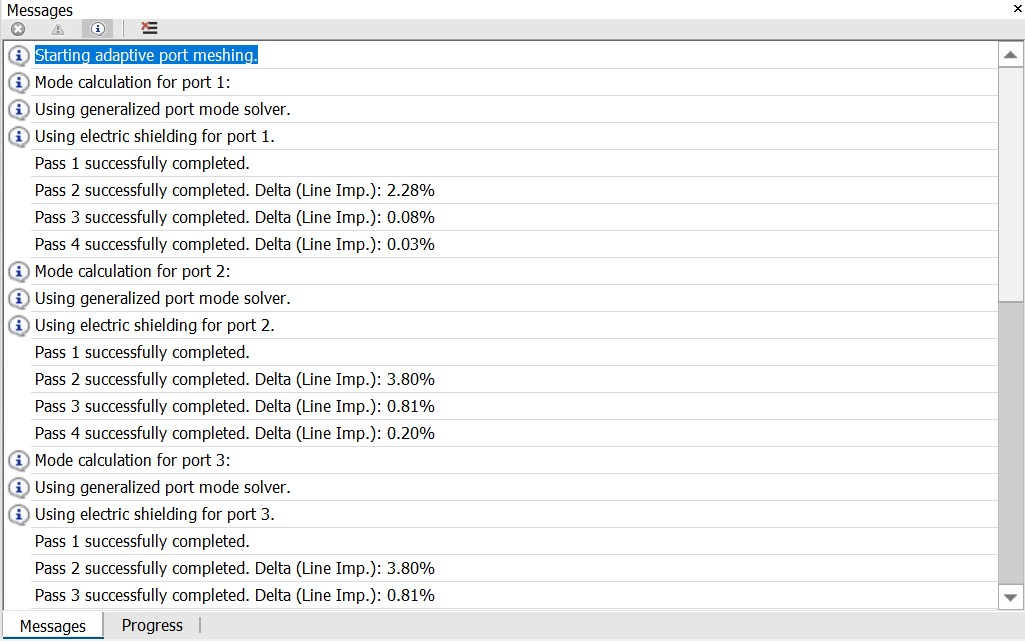
\includegraphics[width=9cm,height=4.4cm]{imagenes/img13}
    \caption{Mensaje de Consola de Simulación.}
    \label{fig:modelamiento8}
\end{figure}
\vspace{10mm}
\begin{figure}[h]    
    \centering
    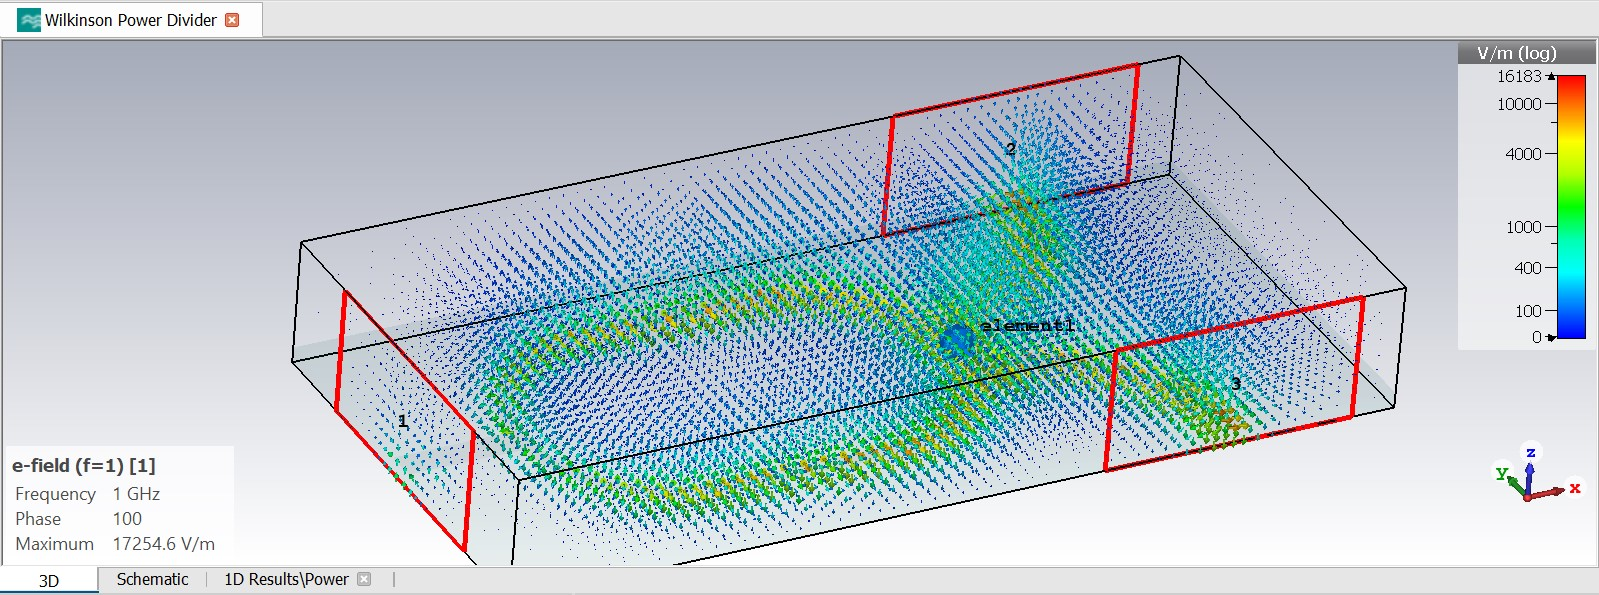
\includegraphics[width=9cm]{imagenes/img15}
    \caption{Vista de Campo Eléctrico.}
    \label{fig:modelamiento9}
\end{figure}
\begin{figure}[h]    
    \centering
    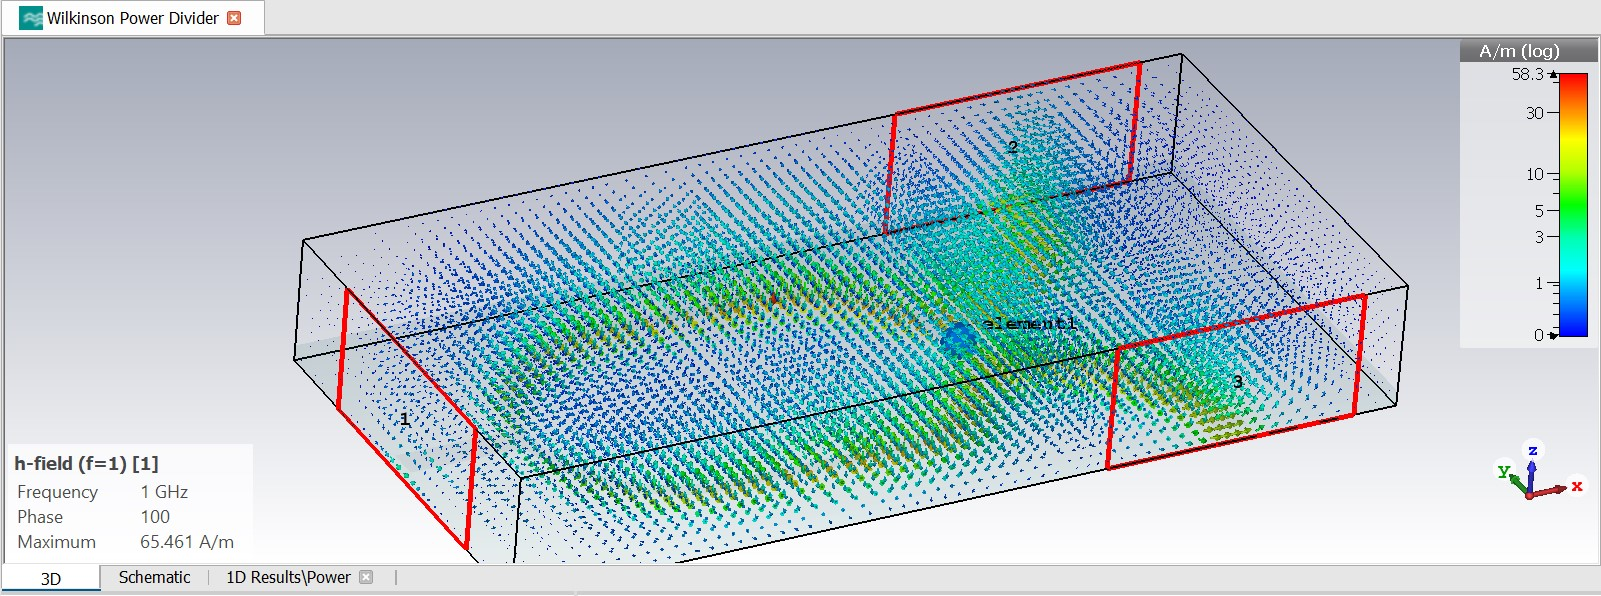
\includegraphics[width=9cm]{imagenes/img16}
    \caption{Vista de Campo Magnético.}
    \label{fig:modelamiento10}
\end{figure}
\section{Conclusiones}
Podemos concluir que en el caso de los puertos 2 y 3 del divisor sean excitados simultaneamente, la matriz de dispersión nos indica que la red es reciproca, esto quiere decir que este divisor puede ser usado tambien como combinador de potencia, las señales de entrada se combinarian dando una resultante en el puerto 1 \cite{wilkinson1960n}.

\begin{figure}[h]    
    \centering
    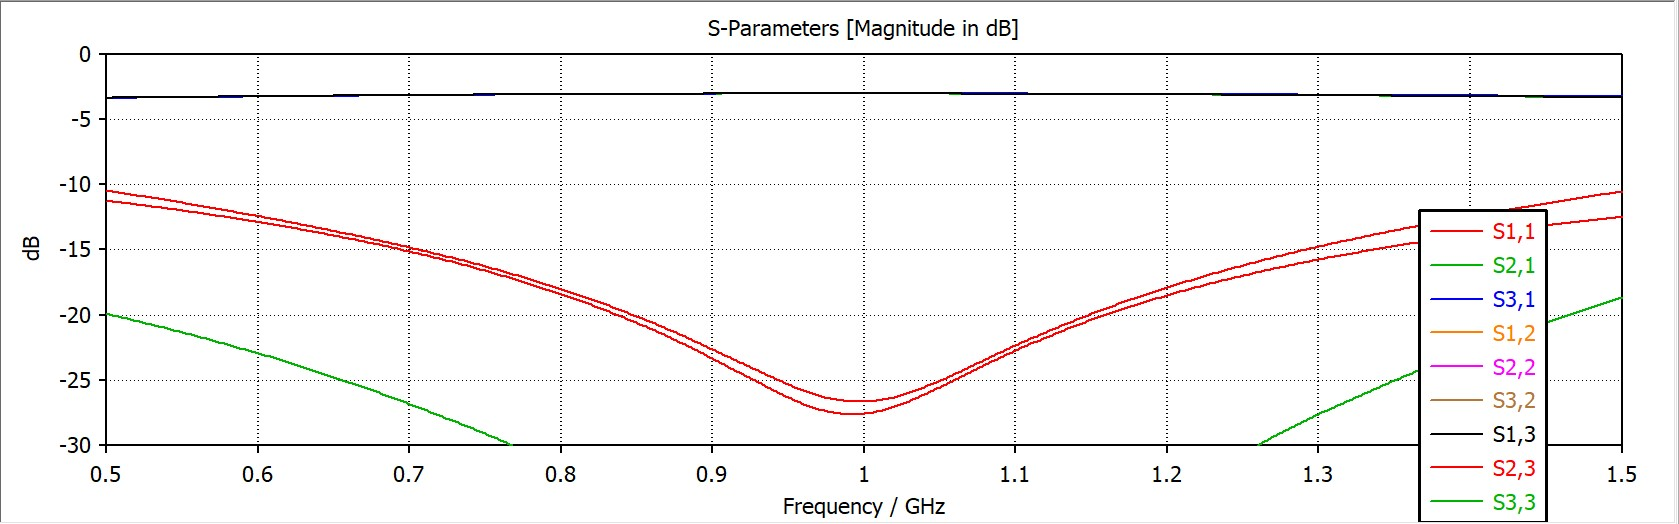
\includegraphics[width=9cm,height=5cm]{imagenes/img18}
    \caption{S Parameters.}
    \label{fig:parametro_s}
\end{figure}

Podemos ver en las curvas de los parametros de dispersión las caracteristicas de la matriz dada en el fundamento teórico, los parametros $S_{31},S_{21}$ que al ser iguales nos dicen que una division igual de potencia fue alcanzada.
Tambien se puede apreciar que os terminales de salida estan aislados esto se puede ver en la gráfica de los parametros $$S_{31},S_{21}$$ 

En la realización de esta simulación, se ha podido observar el fenomeno de división de potencia de este divisor, se entendieron conceptos los conceptos de matriz de dispersión, análisis par-impar, asi como tambien, el uso a un nivel básico de la herramienta de simulación CST Studio Suite.
%\vspace{10mm}
\bibliographystyle{ieeetr}
\bibliography{bibliografia}
\end{document}